\chapter{Christologie dans la Chine du VIIIème siècle à travers le Stèle de Xi'an}

\label{ch:christologieChine}
Rédaction d’une dissertation de 8 pages Vous choisissez une question
montrant comment la christologie est interrogée par une culture/autre tradition
religieuse. Vous travaillez en vous appuyant sur un article ou un autre texte.
Votre sujet et le texte doivent être au préalable validés par le professeur. Votre
travail écrit doit être déposé sur l’ENT (espace dédié) et la date limite pour la
remise de votre travail est le 8 mai 2022
Alternative regarder une approche christologique dans une culture, par exemple
perse ou chinoise. bien montrer la culture chinoise et comment elle s’adapte à
cette ”langue”, cette culture.
\section{Introduction}


Comment la christologie est interrogée par la culture chinoise au VIIIème siècle, à travers la stèle de Xi'an.

\begin{quote}
Si les tous premiers textes que nous possédons se contentent de raconter l'histoire du Messie, il fallut bien, un jour en venir à une présentation du message chrétien dans des catégories et des perspectives proprement chinoises. C'est ce que nous fait comprendre le texte de la Stèle de Xi'an composé en 781, soit environ cent quarante ans après l'arrivée des premiers moines syro-orientaux, en 635. 
Le texte de l'inscription de la Stèle manifeste une vraie synthèse théologique qui puisait dans les trois traditions en présence, christianisme, taoïsme et bouddhisme. \cite[p.~150]{Raguin:JesusMessieXian} 
\end{quote}

\section{Contexte et Structure de la Stèle}
 \paragraph{Une culture Chinoise en plein épanouissement} Si l'empire Tang est souvent présenté comme un « âge d'or » de la civilisation chinoise aussi bien par ses accomplissements militaires que culturels, il le doit à son premier siècle et demi d'existence. Héritière des premiers empires (Qin et Han) ainsi que des évolutions marquées de la période de division (les « Six dynasties »), la dynastie Tang est caractérisée par un État très centralisé, dominé politiquement, économiquement et culturellement par sa capitale Chang'an (actuelle Xi'an, où a été retrouvée la Stèle), une armée divisée entre des troupes frontalières et des troupes de la capitale composées d'une grande partie de « Barbares », et la prépondérance sociale d'un nombre limité de grandes familles.
 Très ouvert aux religions étrangères, le Royaume se referma  : en 830-840, 50 ans après l'écriture de la Stèle, les mesures de répression des religions étrangères sont prises avec un arrière-fond xénophobe : interdiction de contact entre les Chinois et les étrangers en 836, et interdiction de leurs religions en 845. La présence chrétienne en Chine disparut progressivement, d'autant plus que la source perse perdait de la vitalité par la conquête arabe.
 
\paragraph{Historique de la stèle}
le
premier prêtre nestorien à se présenter à Chang'an en 635, un
certain Aluoben ou Alopen, y fut reçu avec des honneurs dignes d'un ambassadeur. L'empereur lui demanda d'écrire un texte qui présente la foi chrétienne, dont on a conservé la trace. Il put créer un monastère avec 21 moines. 
La stèle fut écrite 150 ans plus tard, en 781, retrouvé dans le quartier des marchands de Chang'an. Cette stèle, redécouverte au XVII, est connue selon de nombreux noms, du fait des différentes prononciations du Chang'an : Inscription nestorienne (\cite{saeki:nestorianDocumentsChine}), Inscription , la stèle est écrite à Xi'an et elle présente la foi chrétienne de façon bien différente du texte écrit 150 ans auparavant, du fait d'un travail théologique d'acculturation important. 


\paragraph{Une stèle écrite en excellent Chinois}, signe d'une compréhension fine de la culture chinoise. On pense qu'elle fut écrite par le moine perse et évêque de Chine \textit{Adam},  King-Tsing pour son nom de religion chinois signifiant \textit{lumière et pureté}. Il faut très probablement aidé dans sa tâche, aidé par un lettré chinois. \cite[p.~5]{Havret:stelechretienne}

\paragraph{Une vraie Christologie en contexte chinois} Par rapport à l'exposé de la foi fait par les premiers moines en Chine et dont on a conservé la trace, le texte montre une compréhension beaucoup fine de la culture chinoise : ce n'est pas une simple traduction mais une vraie christologie chinoise.

\paragraph{Titre}
traduction  \cite{Havret:stelechretienne}
\begin{figure}[h!]
    \centering
    \sidecaption{Titre de l'inscription \cite{Pauthier:linscriptionSinganfou} Monument (rappelant) la propagation à travers l'Empire du Milieu de l'Illustre (King) Religion du Ta-ts'in}
    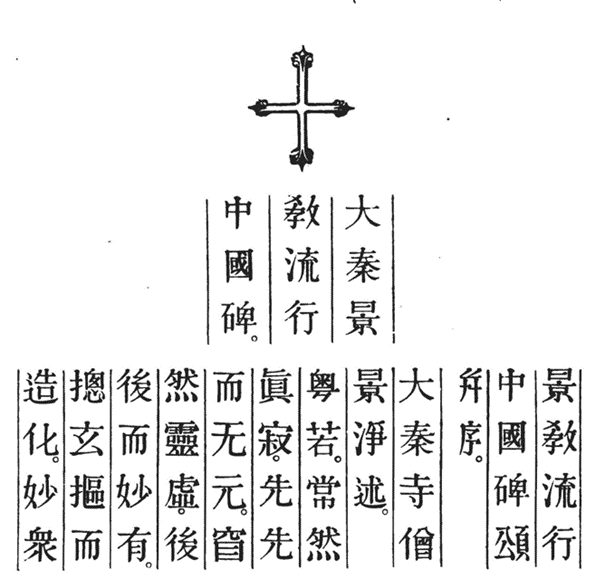
\includegraphics[width=\textwidth]{ChristologieCultureHistoire/Images/PremierParagrapheStele.png}
 
    \label{fig:my_label}
\end{figure}
\paragraph{Un découpage proposé en 25 sections} La stèle peut être découpé en 25 sections, la première sur les attributs de Dieu, puis les trois suivantes sur la Création et la Chute de l'homme (surtout pour développer l'idée d'un homme bon avant la chute par l'orgueil), puis les deux suivantes sur le Christ. A partir de la section 8, on trouve les caractéristiques de la religion, le baptême, les moines, l'éthique, puis plusieurs sections sur l'histoire des chrétiens en Chine. Nous nous concentrerons sur les premières sections et en particulier les section 6 et 7 proprement christologiques.  

\paragraph{Une christologie d'en haut} un développement sur le mal. 

\subsection{la partie proprement Christologique}




\section{Adaptation à la culture Chinoise}

\subsection{Adaptation}

\paragraph{de nombreux éléments  }
\begin{quote}
    dangereux rapprochements [avec la culture Taoiste] (p.21)
\end{quote}
\cite{Havret:stelechretienne}


\paragraph{Hérésie Nestorienne ?} Quelle est la foi enseignée aux Chinois ? Certains (\cite{Gernet:Stele},...), n'hésitent pas à parler de l'hérésie Nestorienne. Il faudrait alors faire attention que ce que nous considérons comme \textit{adaptation au contexte chinois} ne soit en fait que la vision nestorienne du christianisme ou du moins à la perse. Nous prenons comme hypothèse que l'influence nestorienne ne doit pas être surestimée : face à une culture chinoise forte et ancienne, les différences nestoriennes par rapport à la foi orthodoxes apparaissent comme de deuxième ordre. Par ailleurs la foi Chrétienne perse nous est assez largement inaccessible (voir néanmoins \cite{Amir:CoranHistoriens}  : mixité culturelle, importance du terreau judeo chrétien, affirmation des différences avec Bysance pour montrer autonomie) 

\paragraph{Chute, baptême} importance de l'humilité

 \subsection{\textit{ce qui résiste à la culture Chinoise}}

